% kuleuventheme2poster by Janez Kren, June 2018, janez.kren@kuleuven.be

\documentclass{beamer}
\usepackage[orientation=portrait,size=a0,scale=1.4,debug]{beamerposter}
% BEAMERPOSTER OPTIONS:
%	orientation= portrait / landscape
%	size= a0 / a2 / a3 / a4
%	scale = change the size of text (e.g. 1.4 increases all fonts by factor of 1.4)


\usetheme[white,kul]{kuleuven2poster}
% THEME OPTIONS 
%	for logo:   kul (default) / kulak / lrd
%	background colour:   blue (default) / white
%	background sedes logo:   no (default) / sedes
%  e.g. [lrd,white,sedes]


% USE YOUR BACKGROUND IMAGE (optional):
%\titlegraphic{ \includegraphics[height=0.9\paperheight]{mybackground.jpg} } %or, depending on the size: [width=\paperwidth]
%\def\backgdopacity{0.25}  % background image opacity fraction (0=transparent, 1=full colour)


\usepackage[utf8]{inputenc}
\usepackage{ragged2e}  % enables \justifying
\usepackage{booktabs}
\usepackage{multirow}
\renewcommand{\familydefault}{\rmdefault}
\usepackage{xcolor}
\usepackage{hyperref}
\hypersetup{
     colorlinks   = true,
     citecolor    = kul-blue
}
\usepackage{array}
\newcolumntype{C}[1]{>{\centering\let\newline\\\arraybackslash\hspace{0pt}}m{#1}}
\usepackage[sort&compress,numbers]{natbib}

% INFO 
\title{Enumeration of large four-and-two-level designs}
\author{\large Alexandre Bohyn$^{1*}$, Eric Schoen$^{1}$ and Peter Goos$^{1,2}$ }
\institute{\large $^1$KU Leuven $^2$University of Antwerp}
\date{}
 

\begin{document}
\csname beamer@calculateheadfoot\endcsname %recalculate head and foot dimension

\begin{frame}[t]

%%
%%  TITLE (optional)
%%
\vspace{2.5\baseh} % extra vertical space

\begin{tikzpicture}
\node [text width=\textwidth, text ragged, inner sep=0pt, outer sep=0, kul-blue, font=\bfseries\sffamily\fontsize{0.4\baseh pt}{2}\selectfont] 	
{ \inserttitle } ;
% This will create title larger than \Huge. Replace with the line below, to make it smaller or fine-tune.
\end{tikzpicture}

%\textcolor{kul-blue}{\bfseries \Huge \inserttitle}



%%
%% BODY
%%
\vspace{.4\baseh}
\begin{columns}[t]
%COLUMN 1
	\begin{column}{.49\textwidth}
	\justifying
	{\color{kul-blue} \sffamily \large Introduction}
	
    Four-level factors are useful:
	    \begin{itemize}
	        \item to study multi-level categorical factors
	        \item to study non-linear effects of numerical factors
	    \end{itemize}
	~\\
    Current catalogs of four-and-two-level designs:
	    \begin{itemize}
	        \item \textbf{Wu \& Zhang (1993; \cite{wu_minimum_1993}):} 16 and 32-run designs, 1 or 2 four-level factors, up to 11 two-level factors 
	        \item \textbf{Ankenman (1999; \cite{ankenman_design_1999}):} 16 and 32-run designs, 1, 2 or 3 four-level factors, up to 14 two-level factors 
	    \end{itemize}
	    
	\vspace{24pt}
	
	\begin{exampleblock}{\sffamily \large Cheese-making experiment}
	\textbf{Screening experiment in 128 runs}.
	There are 10 potentially influential factors :
	\begin{itemize}
	    \item 9 two-level factors $\rightarrow$ $\mathrm{2^9}$
	    \item 1 four-level factor $\rightarrow$ $\mathrm{4^1}$
	\end{itemize}
	
	\begin{figure}
		\centering
		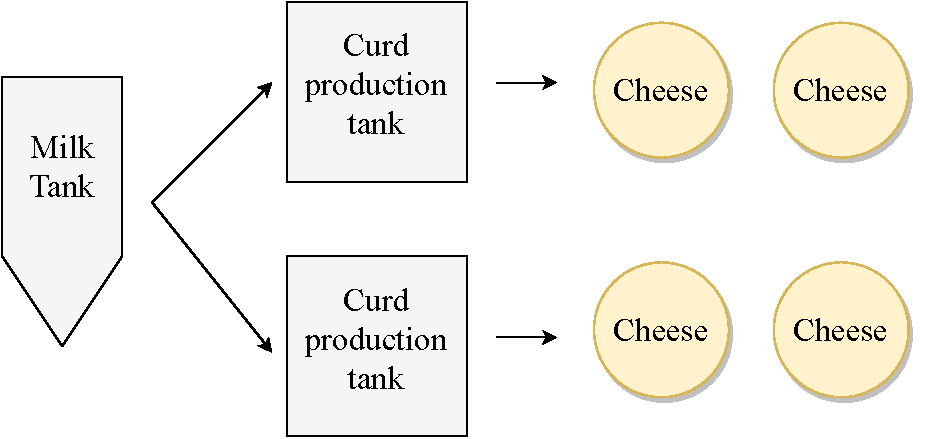
\includegraphics[width=0.9\textwidth]{figures/diagrams-horizontal_no-header.pdf}
	\end{figure}
	
	{\color{red} \large No available catalog !}
	\end{exampleblock}
	
	\vspace{24pt}
	
	\begin{alertblock}{\sffamily \large Goal}
	    Create a {\color{kul-blue}\underline{complete}} catalog of regular four-and-two-level designs with {\color{kul-blue}\underline{large run sizes}}
    	\begin{itemize}
    	    \item {\color{kul-blue} Complete:} all non-equivalent designs
    	    \item {\color{kul-blue} Large run sizes:} for up to 256 runs
    	\end{itemize}
	\end{alertblock}
	
	\vspace{24pt}
	
	{\sffamily \color{kul-blue} \large Methodology}
	\vspace{24pt}
    \begin{figure}
		\centering
		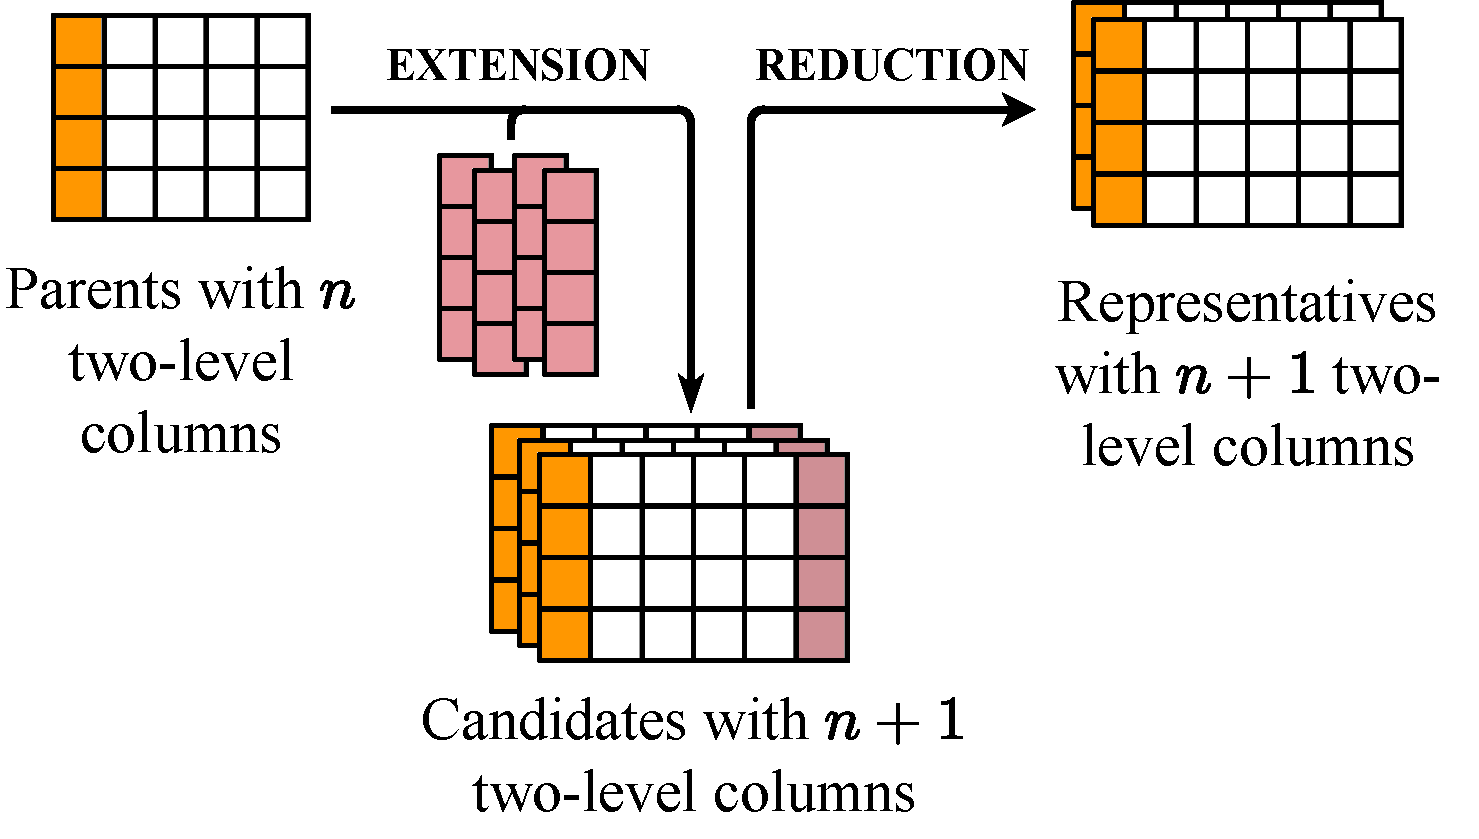
\includegraphics[width=\textwidth]{figures/procedure3.pdf}
    \end{figure}
    
	\end{column}


% COLUMNS 2
	\begin{column}{.49\textwidth}
	\justifying
    {\color{kul-blue} \sffamily \large Selected algorithms}
    \begin{itemize}
        \item Extension procedures: Search Table (ST; \cite{bingham_minimum-aberration_1999}) , Delete-One-Factor Projection (DOP; \cite{xu_algorithmic_2009}), Minimum Complete Set (MCS; \cite{schoen_complete_2010}) 
        \item Reduction procedures: NAUTY graph isomorphism \cite{ryan_minimum_2010,mckay_practical_2014}, LMC canonical form testing \cite{schoen_complete_2010}
    \end{itemize}
        
    \vspace{24pt}    
        
    % Table generated by Excel2LaTeX from sheet 'Tabelle1'
\begin{table}[htbp]
  \centering
    \begin{tabular}{lccc}
      & \multicolumn{1}{c}{\textbf{ST}} & \multicolumn{1}{c}{\textbf{DOP}} & \multicolumn{1}{c}{\textbf{MCS}} \\
    \midrule
    \textbf{NAUTY} & ST-NAUTY & DOP-NAUTY & \textcolor[rgb]{ 1,  0,  0}{Not optimal} \\
    \textbf{LMC test} & \textcolor[rgb]{ 1,  0,  0}{Not optimal} & \textcolor[rgb]{ 1,  0,  0}{Incompatible} & MCS - LMC \\
    \bottomrule
    \end{tabular}%
  \label{tab:selected_procedures}%
\end{table}%

        
    \vspace{24pt}
        
	\begin{figure}
    	\centering
    	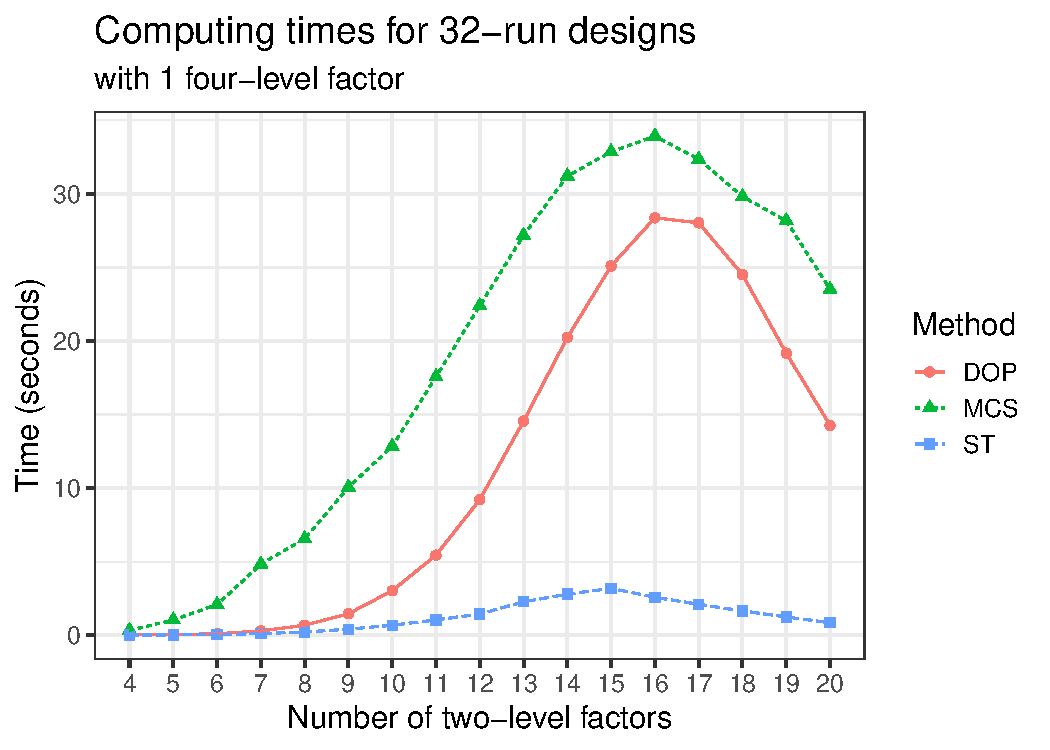
\includegraphics[width=0.9\textwidth]{figures/plot.pdf}
	\end{figure}
    	
	\begin{itemize}
	    \item ST-NAUTY was the most efficient of the 3 enumeration methods. Similar results for other test cases.
	\end{itemize}
    	
    \vspace{24pt}
	
	{\color{kul-blue} \sffamily \large Results}
	
	Number of enumerated $\mathrm{4^m2^n}$ designs for $\mathrm{n \leq 20}$:
	
	% Table generated by Excel2LaTeX from sheet 'Tabelle1'
\begin{table}[htbp]
  \centering
    \begin{tabular}{C{2cm}C{6cm}C{6cm}C{6cm}C{6cm}}
    \multirow{2}{2cm}{\textbf{m}} & \multicolumn{4}{c}{\textbf{N} (Resolution)} \\
    \cmidrule{2-5} & \textbf{32} $\mathrm{(III)}$ & \textbf{64} $\mathrm{(IV)}$ & \textbf{128} $\mathrm{(IV)}$ & \textbf{256} $\mathrm{(IV)}$\\
    \midrule
    \textbf{1} & 8,279 & 254 & 1,442,301 & $>$ 86,528 \\
    \textbf{2} & 36,692 & 137 & 2,837,275 & $>$ 40,848 \\
    \textbf{3} & - & 28 & 2,141,911 & $>$ 78,386 \\
    \bottomrule
    \end{tabular}%
  \label{tab:number_ni_designs}%
\end{table}%

	
	\vspace{24pt}
	
	\begin{exampleblock}{\color{kul-blue} \sffamily \large Cheese-making experiment revisited}
	There are 264 $\mathrm{4^12^9}$ designs involving 128 runs

	% Table generated by Excel2LaTeX from sheet 'ma_designs'
\begin{table}[htbp]
  \centering
    \begin{tabular}{C{3cm}C{10cm}C{10cm}}
    \textbf{ID} & \textbf{Added columns} & \textbf{WLP} $\mathrm{(A_4,A_5,A_6)}$ \\
    \midrule
    1 & 60, 77, 86, 103 & (0, 8, 6) \\
    2 & 29, 46, 90, 101 & (0, 9, 3) \\
    3 & 13, 58, 91, 116 & (1, 6, 6) \\
    \bottomrule
    \end{tabular}%
  \label{tab:addlabel}%
\end{table}%


	\begin{itemize}
	    \item Designs 1 and 2 were not compatible with required restrictions in the randomization.
	    \item Design 3 is the best design that is compatible with these restrictions.
	    \item Remaining designs have inferior WLP.
	\end{itemize}
    \end{exampleblock}
	\end{column}
	
\end{columns}
    
    %\vspace{10pt}
    \begin{columns}
    \begin{column}{1.07\textwidth}
    \begin{block}{\color{kul-blue} \sffamily \large References}
	\scriptsize
	\bibliographystyle{unsrt}
	\bibliography{references}
	\end{block}
	\hfill 
	$^{*}$\href{mailto:alexandre.bohyn@kuleuven.be}{alexandre.bohyn@kuleuven.be}
	\end{column}
	\end{columns}
    
\end{frame}
\end{document}
